\documentclass[11pt,twoside,a4paper]{article}
% http://www-h.eng.cam.ac.uk/help/tpl/textprocessing/latex_maths+pix/node6.html symboles de math
% http://fr.wikibooks.org/wiki/Programmation_LaTeX Programmation latex (wikibook)
%=========================== En-Tete =================================
%--- Insertion de paquetages (optionnel) ---
\usepackage[french]{babel}   % pour dire que le texte est en fran{\'e}ais
\usepackage{a4}	             % pour la taille   
\usepackage[T1]{fontenc}     % pour les font postscript
\usepackage{epsfig}          % pour gerer les images
%\usepackage{psfig}
\usepackage{amsmath, amsthm} % tres bon mode mathematique
\usepackage{amsfonts,amssymb}% permet la definition des ensembles
\usepackage{float}           % pour le placement des figure
\usepackage{verbatim}

\usepackage{longtable} % pour les tableaux de plusieurs pages

\usepackage[table]{xcolor} % couleur de fond des cellules de tableaux

\usepackage{lastpage}

\usepackage{multirow}

\usepackage{multicol} % pour {\'e}crire dans certaines zones en colonnes : \begin{multicols}{nb colonnes}...\end{multicols} 

% \usepackage[top=1.5cm, bottom=1.5cm, left=1.5cm, right=1.5cm]{geometry}
% gauche, haut, droite, bas, entete, ente2txt, pied, txt2pied
\usepackage{vmargin}
\setmarginsrb{1.0cm}{1.0cm}{1.0cm}{1.0cm}{15pt}{3pt}{57pt}{20pt}

\usepackage{lscape} % changement orientation page
%\usepackage{frbib} % enlever pour obtenir references en anglais
% --- style de page (pour les en-tete) ---
\pagestyle{headings}

% % % en-tete et pieds de page configurables : fancyhdr.sty

% http://www.trustonme.net/didactels/250.html

% http://ww3.ac-poitiers.fr/math/tex/pratique/entete/entete.htm
% http://www.ctan.org/tex-archive/macros/latex/contrib/fancyhdr/fancyhdr.pdf
\usepackage{fancyhdr}
\pagestyle{fancy}
% \newcommand{\chaptermark}[1]{\markboth{#1}{}}
% \newcommand{\sectionmark}[1]{\markright{\thesection\ #1}}
\fancyhf{}
\fancyhead[LE,RO]{\bfseries\thepage}
\fancyhead[LO]{\bfseries\rightmark}
\fancyhead[RE]{\bfseries\leftmark}
\fancyfoot[LE]{\thepage /\pageref{LastPage} \hfill
	blockchain
\hfill 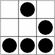
\includegraphics[width=0.5cm]{img/logo_glider.png} }
\fancyfoot[RO]{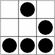
\includegraphics[width=0.5cm]{img/logo_glider.png} \hfill
	blockchain
\hfill \thepage /\pageref{LastPage}}
\renewcommand{\headrulewidth}{0.5pt}
\renewcommand{\footrulewidth}{0.5pt}
\addtolength{\headheight}{0.5pt}
\fancypagestyle{plain}{
	\fancyhead{}
	\renewcommand{\headrulewidth}{0pt}
}

%% \pagestyle{empty}

\renewcommand{\headrulewidth}{0.25pt}
\renewcommand{\footrulewidth}{0.5pt}
%% \setlength{\headheight}{85pt}
% \addtolength{\headheight}{0.5pt}
% \fancypagestyle{plain}{
% 	\fancyhead{}
% 	\fancyfoot{}
% 	\renewcommand{\headrulewidth}{0pt}
% }

%--- Definitions de nouvelles commandes ---
\newcommand{\N}{\mathbb{N}} % les entiers naturels


%--- Pour le titre ---
\def\maketitle{%
	\begin{center}
		\begin{tabular}[c]{c|c}
			\textsc{\textbf{Institution}}~\\[\baselineskip]~\\[\baselineskip]
			\emph{\textbf{Date 09-09-2009}}~\\[\baselineskip]~\\[\baselineskip]
			\emph{\textbf{Pr{\'e}cisions relatives au contexte}}~\\[\baselineskip]~\\[\baselineskip]
			\textsc{Auteur inestimable}~\\[\baselineskip]~\\[\baselineskip]
			& 
			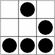
\includegraphics[width=3cm]{img/logo_glider.png}~\\[\baselineskip]
		\end{tabular}
		% \\ \hline
		 	% % if more than one logo
			% 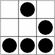
\includegraphics[width=5cm]{img/logo_glider.png}
			% 
\includegraphics[width=5cm]{img/logo_wifi.png}
		% \\ \hline
		% \end{tabular}
			~\\[\baselineskip]~\\[\baselineskip]
			\Huge{Titre principal}~\\[\baselineskip]
			\Large{Titre secondaire}~\\[\baselineskip]
		
		~\\[\baselineskip]
		~\\[\baselineskip]
	\large{
		\textsc{\textbf{Institution d'accueil et jury}}
		~\\[\baselineskip]
		<<titre personne>> : \texttt{Anne ONYME}~\\[\baselineskip]
		<<titre personne>> : \texttt{Jocelyn CONNU}~\\[\baselineskip]
		~\\[\baselineskip]
		\textit{Pr{\'e}cisions du contexte de r{\'e}daction de l'article}
	}

	\end{center}

}%



%--- Pour le glossaire --- a defaut de \makeglossary ou d'utilisation d'index latex

\definecolor{verylightgray}{rgb}{0.8,0.8,0.8}
\def\makeglossaire{%
	\begin{center}

	\begin{tabular}{|>{\columncolor{verylightgray}} p{0.2\textwidth}|p{0.8\textwidth}|}

		\hline

		\textbf{BLAST} & 

			\begin{tabular}{p{0.8\textwidth}}

			Basic Local Alignment Search Tool \\

			\textit{algorithmes et logiciels pour l'alignement de s{\'e}quences et la recherche de similarit{\'e}s locales}

			\end{tabular} \\

		\hline

		\textbf{BNDB} & Biochemical NetWork DataBase \textit{(entrep{\^o}t de donn{\'e}es)} \\

		\hline

	\end{tabular}

\end{center}

}%

%============================= Corps =================================
\begin{document}
%ecrire le titre...
%% \maketitle
%% \setcounter{page}{0}
%% \thispagestyle{empty}
%% \clearpage

%% \setcounter{page}{0}
%% \thispagestyle{empty}

\setlength\parindent{0pt}

\texttt{\small https://www.letemps.ch/economie/2015/11/06/blockchain-promet-une-nouvelle-revolution }~\\

\textbf{\Large La blockchain promet une nouvelle r{\'e}volution}~\\
\emph{Emmanuel Garessus -- Publi{\'e} vendredi 6 novembre 2015 {\`a} 14:07, modifi{\'e} vendredi 6 novembre 2015 {\`a} 14:27.}~\\

\textbf{La nouvelle technologie du partage, une forme de registre des transactions num{\'e}rique s{\^u}re et infalsifiable, permet de r{\'e}duire les co{\^u}ts, d'am{\'e}liorer la qualit{\'e} et la vitesse des services. Son impact devrait {\^e}tre fort en finance, dans l'immobilier et m{\^e}me dans le syst{\`e}me {\'e}lectoral. }~\\

<<L'emploi de la blockchain dans l'{\'e}conomie promet de r{\'e}volutionner l'immobilier (en cr{\'e}ant un nouveau registre foncier num{\'e}rique), les services financiers, le syst{\`e}me de vote, le commerce des biens de luxe et l'administration fiscale>>, d{\'e}clare Andreas Lenzhofer, expert en blockchain aupr{\`e}s de PwC Strategy\&. ~\\

Cette technologie n'est pas vraiment nouvelle puisque le bitcoin, la monnaie virtuelle, s'appuie sur le m{\^e}me principe, mais <<ce n'est qu'apr{\`e}s l'{\'e}clatement de la bulle du bitcoin que l'on a vraiment compris le formidable potentiel de la blockchain>>, poursuit l'expert. <<Ce bouleversement est rendu possible par son extraordinaire pouvoir de d{\'e}sinterm{\'e}diation>>, fait valoir le magazine The Economist dans un dossier sur ce th{\`e}me. <<La blockchain est une machine {\`a} cr{\'e}er de la confiance>>, affirme l'hebdomadaire britannique. Au lieu de faire confiance {\`a} l'interm{\'e}diaire neutre habituel, qu'il s'agisse du notaire (transmission d'immeubles), du gouvernement (vote, imp{\^o}ts) ou du banquier (transfert de titres ou d'argent), la confiance est transf{\'e}r{\'e}e {\`a} la machine, puisque la technologie est enti{\`e}rement s{\^u}re, affirme le magazine. ~\\

\textbf{Un stockage num{\'e}rique}~\\

La blockchain -- le terme n'a pas de traduction fran\c{c}aise -- se d{\'e}finit par <<une technologie de stockage num{\'e}rique et de transmission {\`a} co{\^u}t minime, d{\'e}centralis{\'e}e et totalement s{\'e}curis{\'e}e>>, selon le site Blockchain France (https://blockchainfrance.wordpress.com/). Concr{\`e}tement, il s'agit d'un livre de compte -- un registre num{\'e}rique -- contenant la liste de tous les {\'e}changes effectu{\'e}s entre les utilisateurs depuis sa cr{\'e}ation. Ce registre, potentiellement utile dans l'immobilier, l'art et les biens de luxe, constitue un historique infalsifiable des {\'e}changes de personne {\`a} personne. Pour hacker une blockchain ou la manipuler, il faudrait avoir acc{\`e}s et modifier au m{\^e}me moment des dizaines de milliers de bases de donn{\'e}es ind{\'e}pendantes les unes des autres. ~\\

\begin{minipage}[h]{0.75\textwidth}
	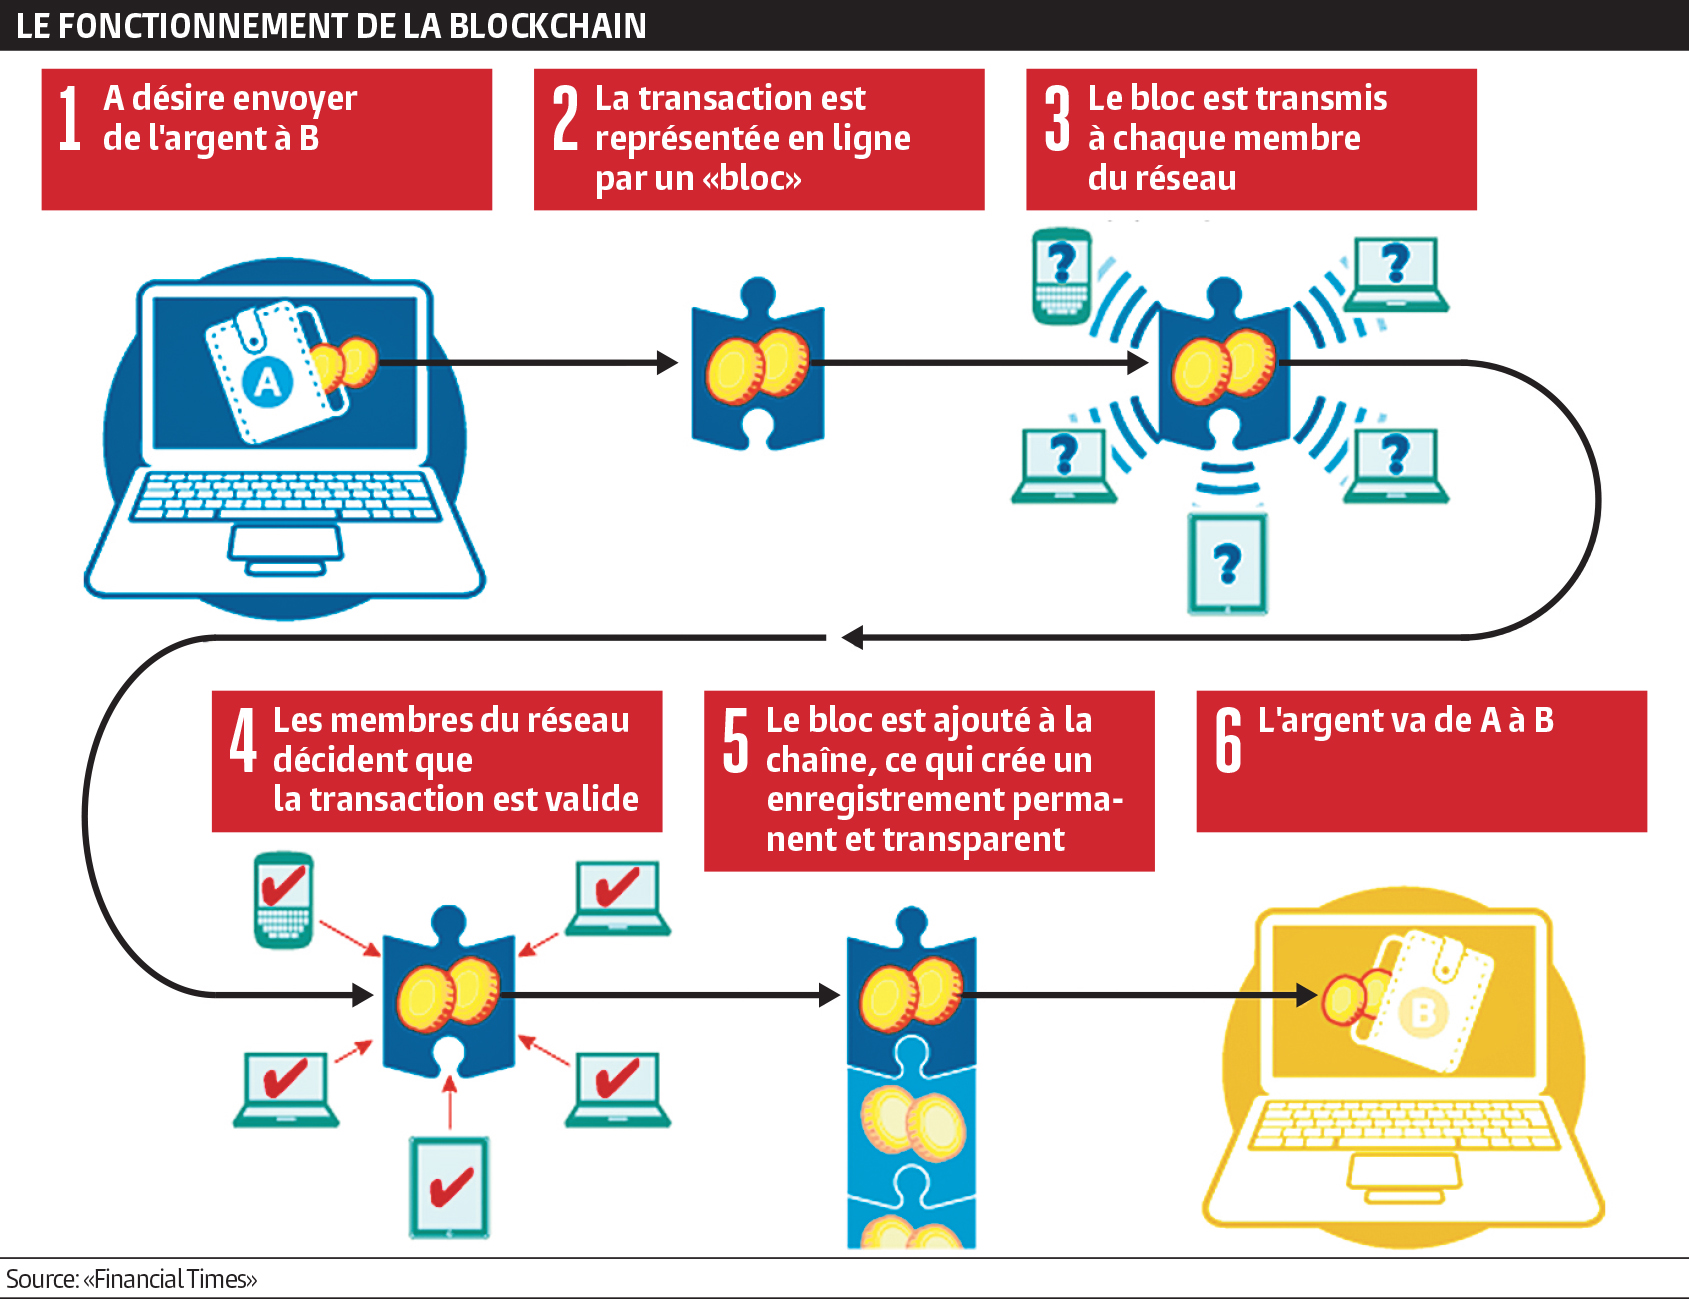
\includegraphics[width=0.95\textwidth]{img/L17_Blockchain258_0.jpg}
\end{minipage} \hfill \begin{minipage}[h]{0.23\textwidth}
	\textbf{Infographie. }Comment fonctionne le blockchain?~\\

	Cette technologie rappelle les facteurs de disruption tels qu'Uber, puisqu'elle repose sur les m{\^e}mes principes de d{\'e}centralisation, de partage et d'utilisation d'Internet. Mais elle est r{\'e}volutionnaire, puisqu'elle concernera toutes les branches qui font appel {\`a} un interm{\'e}diaire. Elle int{\`e}gre aussi les facteurs de tra\c{c}abilit{\'e} des informations et de d{\'e}centralisation. ~\\
\end{minipage} ~\\~\\

Une start-up fran\c{c}aise, Synereo, entend devenir <<le nouveau Facebook>>, mais en utilisant la blockchain. Mais autant Facebook concentre les informations {\`a} son seul profit, autant l'entreprise de Dor Konforty, son patron, place l'utilisateur au centre de son mod{\`e}le. La valeur des informations ne se retrouve pas dans le b{\'e}n{\'e}fice de l'entreprise mais, gr{\^a}ce {\`a} la blockchain, dans celle des utilisateurs. Ces derniers sont cens{\'e}s reprendre le contr{\^o}le de leur identit{\'e}. Synereo entend <<valoriser la s{\'e}curit{\'e} et la vie priv{\'e}e plut{\^o}t que le profit>>, selon Blockchain France. Elle dispose d'un fil d'actualit{\'e}, d'une liste d'amis, et elle permet, {\`a} la diff{\'e}rence de Facebook, de g{\'e}rer l'attention port{\'e}e {\`a} des personnes et des id{\'e}es. Elle utilise en effet des <<variables d'attention>>, en fonction de la pertinence des contenus et du partage des informations. L'une de ces variables, unit{\'e} de mesure de l'attention, est appel{\'e}e <<reo>>. Une personne {\'e}loign{\'e}e de votre r{\'e}seau vous apporte davantage de <<reo>> que si elle vous est proche. ~\\

De nombreuses branches y d{\'e}c{\`e}lent un fort potentiel. Les start-up pullulent, autant dans la musique que dans l'{\'e}ducation ou les donn{\'e}es m{\'e}dicales. Orange a annonc{\'e} en septembre investir des millions de dollars dans cette technologie. ~\\

<<Les grandes soci{\'e}t{\'e}s suisses, par exemple les grandes banques, en vertu de la capacit{\'e} de la blockchain de changer profond{\'e}ment le syst{\`e}me financier, sont tr{\`e}s pr{\'e}sentes dans le d{\'e}veloppement de cette technologie, les autres sont plus attentistes>>, observe Andreas Lenzhofer. Le trafic des paiements comporte en effet de nombreuses {\'e}tapes permettant de s'assurer du bon fonctionnement de l'op{\'e}ration. Il en va de m{\^e}me de l'achat et de la vente d'actions en bourses. Il suffit de mentionner les fonctions d'administration, de r{\`e}glement et de compensation. Avec la blockchain, il sera possible de supprimer toutes ces fonctions interm{\'e}diaires. <<Le consommateur ou l'investisseur final, ainsi que le grand public, ne s'apercevra de rien, mais toutes les op{\'e}rations effectu{\'e}es en coulisse seront boulevers{\'e}es>>, assure Andreas Lenzhofer. ~\\

\textbf{Investissements des banques}~\\

UBS confirme avoir ouvert ce printemps {\`a} Londres l'UBS Innovation Lab, un laboratoire sur la blockchain dans un centre d'innovation fintech, le Level39. Ce dernier regroupe 170 start-up technologiques. Ce groupe de chercheurs comprend six personnes plac{\'e}es sous la direction d'Alex Batlin. L'une des premi{\`e}res exp{\'e}riences a consist{\'e} {\`a} d{\'e}velopper une <<obligation intelligente>> (smart bond). Il s'agit ici d'{\'e}mettre une obligation en {\'e}liminant les op{\'e}rations d'avant et d'apr{\`e}s n{\'e}goce. UBS a par ailleurs lanc{\'e} un concours, le 12 ao{\^u}t, (The UBS Future of Finance Challenge) qui s'adresse aux entreprises et aux start-up du monde entier. L'id{\'e}e du concours est de trouver des id{\'e}es et des solutions innovantes, voire potentiellement disruptives ou perturbantes, pour accompagner la r{\'e}volution technologique du monde bancaire. UBS collabore par ailleurs avec d'autres incubateurs et acc{\'e}l{\'e}rateurs: Level39, JFDI.Asia, NUS Enterprise @ BLK71 ainsi qu'avec l'agence d'innovations 100\% Open. ~\\

PwC Strategy\& recommande {\`a} ses clients dans un premier temps d'identifier le probl{\`e}me et de l'analyser, d'accompagner le progr{\`e}s technologique, dans un deuxi{\`e}me temps de proc{\'e}der {\`a} des essais pilotes en vertu des opportunit{\'e}s. ~\\
Six Group investit dans cette nouvelle technologie, par l'interm{\'e}diaire de sa division Securites Services. Credit Suisse souhaite positionner la Suisse sur la carte mondiale des fintech. Certains th{\`e}mes financiers s{\'e}lectionn{\'e}s devraient, {\`a} son avis, faire l'objet d'une grande attention, tels la gestion de fortune, la blockchain, la gestion de la s{\'e}curit{\'e} et de l'identit{\'e}. ~\\

La plupart des initiatives peuvent {\^e}tre lues sur le site: etstalkpayments.com/bank-wise-analysis-of-blockchain-activity/. ~\\

Le potentiel industriel est {\'e}vident en termes de baisse des co{\^u}ts. La banque Santander estime {\`a} 20 milliards de dollars par an d'ici {\`a} 2022 le potentiel d'{\'e}conomies de cette technologie. C'est la seule estimation {\`a} ce jour. Mais le potentiel ne s'arr{\^e}te pas l{\`a}. La blockchain permet aussi une am{\'e}lioration dans la qualit{\'e} du service, puisqu'elle exclut le risque de fraude, et rend toutes les transactions beaucoup plus rapides, puisqu'il n'est plus n{\'e}cessaire d'attendre trois jours pour avoir la confirmation de la vente d'un titre financier.~\\

{\`A} propos de l'auteur ~\\
Emmanuel Garessus --- @garessus ~\\
Mes int{\'e}r{\^e}ts: innovation, finance, philosophie et football (avec un penchant pour le FC B{\^a}le). ~\\

%% \begin{minipage}[h]{5.00cm}
%% 	
\includegraphics[width=4.85cm]{img/pacman.png}
%% \end{minipage} \hfill \begin{minipage}[h]{13cm}
%% 	\texttt{Marc Andreessen}~\footnotemark, concepteur du premier navigateur graphique, \texttt{Mosaic}~\footnotemark, et d{\'e}sormais l'un des plus influents \texttt{\emph{venture capitalists}}~\footnotemark du march{\'e}, a pour habitude de d{\'e}clarer que <<\emph{le logiciel d{\'e}vore le monde}>>. Il a explicit{\'e} sa formule dans un \texttt{article}~\footnotemark paru l'ann{\'e}e derni{\`e}re dans le \emph{Wall Street Journal} : l'{\`e}re du \emph{pure playing} est termin{\'e}e ; d{\'e}sormais le logiciel va s'immiscer dans tous les secteurs de l'{\'e}conomie, s'hybrider avec le mat{\'e}riel et affecter les positions et les niveaux de marge de tous les acteurs en place.
%% \end{minipage} ~\\~\\
%% \footnotetext[1]{\texttt{http://en.wikipedia.org/wiki/Marc\_Andreessen}}
%% \footnotetext[2]{\texttt{http://en.wikipedia.org/wiki/Mosaic\_(web\_browser)}}
%% \footnotetext[3]{\texttt{http://a16z.com/}}
%% \footnotetext[4]{\texttt{http://online.wsj.com/article/SB10001424053111903480904576512250915629460.html}}

%% ~\\

\clearpage

\texttt{\small http://blog.d2-si.fr/2016/01/19/blockchain/}~\\

\textbf{\Large Le Blockchain, nouveau maillon fort de l'{\'e}conomie num{\'e}rique}~\\
\emph{19/01/2016 -- by Nicolas P{\'e}ray -- in D{\'e}couvrir, Experts D2SI, Paroles d'expert. }~\\

%% D2SI_Blog_Image_Blockchain
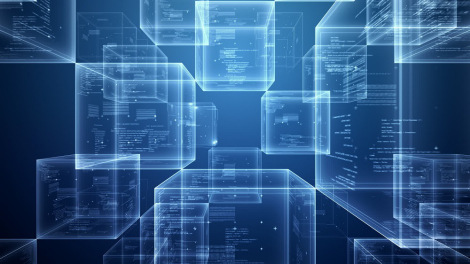
\includegraphics[width=0.95\textwidth]{img/d2si_blog_image_blockchain.jpg}~\\

\textbf{``Blockchain'' : le terme est sur toutes les l{\`e}vres du monde financier. Souvent assimil{\'e}e au sulfureux bitcoin, cette technologie offre des promesses in{\'e}gal{\'e}es en terme de s{\'e}curit{\'e} et d'autonomie. Mais comment fonctionne le blockchain, et quelles sont ses applications ?}~\\
\textbf{Au-del{\`a} du monde de la finance, le blockchain pourrait bien r{\'e}volutionner l'{\'e}conomie en rempla\c{c}ant les tiers de confiance centralis{\'e}s par un syst{\`e}me informatique d{\'e}centralis{\'e}. Explications. }~\\

Le blockchain est un r{\'e}seau constitu{\'e} de milliers d'ordinateurs r{\'e}partis partout dans le monde, qui travaillent en permanence {\`a} la s{\'e}curit{\'e} du syst{\`e}me. Chaque ordinateur stocke une copie des {\'e}changes effectu{\'e}s, et chaque bloc de transaction valid{\'e} est ajout{\'e} au registre, ce qui forme la cha{\^i}ne de blocs.~\\

\textbf{Bitcoin et blockchain}~\\

Prenons l'exemple du bitcoin qui s'appuie sur une blockchain cr{\'e}{\'e}e en 2012. Le principe de base est de rendre inviolable l'historique des transactions stock{\'e}es dans la cha{\^i}ne. Pour ce faire, on va s'appuyer sur le r{\'e}seau d'internet et sur le hachage.~\\
Qu'est-ce que le hachage ? Une \emph{fonction de hachage~\footnote{\texttt{https://fr.wikipedia.org/wiki/Fonction\_de\_hachage}}} prend n'importe quelle donn{\'e}e et la mouline pour en sortir un r{\'e}sultat incompr{\'e}hensible. La particularit{\'e} est que, contrairement au chiffrement dans lequel on peut retrouver les donn{\'e}es initiales gr{\^a}ce {\`a} la bonne clef tenue secr{\`e}te, avec le hachage il est absolument impossible de retrouver les donn{\'e}es initiales. On ne peut aller que dans un sens. Tout ce qu'on sait, c'est que hacher une m{\^e}me donn{\'e}e donnera toujours le m{\^e}me r{\'e}sultat, alors que le moindre petit changement le fait varier enti{\`e}rement. Quel est l'int{\'e}r{\^e}t alors ? Cela sert {\`a} v{\'e}rifier qu'une donn{\'e}e, qui peut {\^e}tre tr{\`e}s volumineuse et complexe, est identique {\`a} un mod{\`e}le en comparant plus simplement les hachages. Par exemple, le hachage est utilis{\'e} pour v{\'e}rifier qu'un t{\'e}l{\'e}chargement s'est bien d{\'e}roul{\'e}. Il suffit de calculer le hachage du fichier, de fa\c{c}on presque instantan{\'e}e, et de le comparer {\`a} celui fourni sur le site, ce qui est infiniment plus rapide {\`a} r{\'e}cup{\'e}rer que le fichier m{\^e}me.~\\

\begin{minipage}[h]{0.49\textwidth}
	%% D2SI_Blog_Image_Blockchain_Hachage
	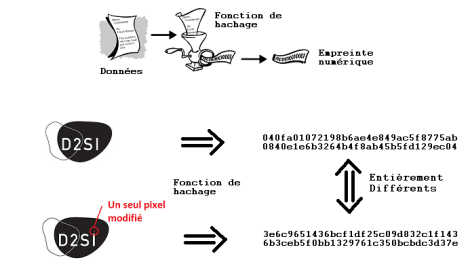
\includegraphics[width=0.95\textwidth]{img/d2si_blog_image_blockchain_hachage1.png}~\\
	%% D2SI_Blog_Image_Blockchain_Chainage
	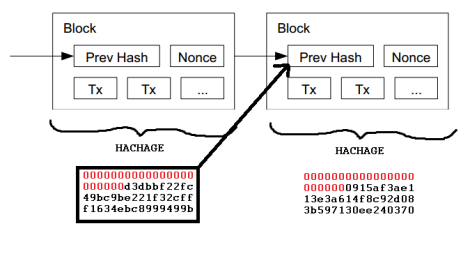
\includegraphics[width=0.95\textwidth]{img/d2si_blog_image_blockchain_chainage.png}
\end{minipage} \hfill \begin{minipage}[h]{0.50\textwidth}
	Comment le hachage est-il exploit{\'e} dans le cas de la blockchain ? Les donn{\'e}es sont verrouill{\'e}es dans un bloc en les compl{\'e}tant de mani{\`e}re suffisamment originale pour que ce soit difficile {\`a} r{\'e}aliser. Concr{\`e}tement, on impose au r{\'e}sultat du hachage de commencer par un grand nombre de z{\'e}ros. Comme ces r{\'e}sultats sont plus rares avec le nombre de z{\'e}ros, il est tr{\`e}s long d'en trouver. En effet, vu que le hachage ne fonctionne que dans un sens, il n'y a pas de solution plus rapide que de g{\'e}n{\'e}rer des caract{\`e}res al{\'e}atoires {\`a} ajouter au bloc de donn{\'e}es, puis de calculer le hachage pour v{\'e}rifier si cela respecte la condition. Sinon il faut trouver d'autres caract{\`e}res et recommencer. Afin de cha{\^i}ner les blocs de donn{\'e}es, et de cr{\'e}er la blockchain proprement dite, on ajoute dans chaque bloc le r{\'e}sultat du hachage pr{\'e}c{\'e}dent. Ainsi, si on modifie un {\'e}l{\'e}ment de la cha{\^i}ne, le r{\'e}sultat du hachage redevient commun (pas de z{\'e}ros) et il faut donc retrouver une bonne combinaison de caract{\`e}res al{\'e}atoires pour le bloc modifi{\'e}, mais {\'e}galement pour tous les suivants par r{\'e}action en cha{\^i}ne sur les variations de valeur des hachages.~\\
\end{minipage}

%% \begin{minipage}[h]{0.24\textwidth}
%% 	%% D2SI_Blog_Image_Blockchain_Chainage
%% 	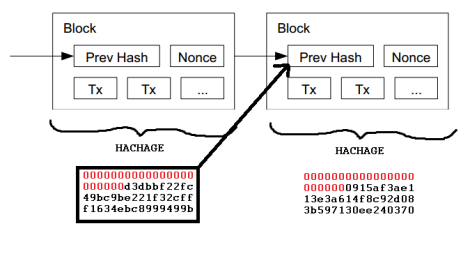
\includegraphics[width=0.95\textwidth]{img/d2si_blog_image_blockchain_chainage.png}
%% \end{minipage} \hfill \begin{minipage}[h]{0.75\textwidth}
	Dans le cas du bitcoin, la difficult{\'e} (le nombre de z{\'e}ros) est r{\'e}gl{\'e}e pour que cette op{\'e}ration prenne 10 minutes en moyenne. Ainsi, tout le r{\'e}seau participant, les ``\textbf{mineurs de bitcoin~\footnote{https://bitcoin.fr/minage/}}'', cherche en permanence, qu'il y ait des transactions ou non, {\`a} ajouter un bloc {\`a} la cha{\^i}ne. Le premier qui y arrive est r{\'e}compens{\'e} par des bitcoins et sa cha{\^i}ne est accept{\'e}e par le reste du r{\'e}seau (car elle est plus longue...) afin de travailler sur le bloc suivant. L'id{\'e}e est qu'un attaquant, pour r{\'e}ussir {\`a} modifier une transaction, ne peut pas passer discr{\`e}tement par une porte d{\'e}rob{\'e}e pour hacker un compte sans que personne ne s'aper\c{c}oive du changement. Il est oblig{\'e} de s'engager frontalement dans une course contre le r{\'e}seau pour le d{\'e}passer en nombre de blocs. Une course qui lui est hautement d{\'e}favorable d{\`e}s l'instant qu'il poss{\`e}de moins de 50% de la puissance de calcul du r{\'e}seau.~\\
%% \end{minipage}

\textbf{La fiabilit{\'e} du syst{\`e}me Bitcoin ?} %% ~\\

Est-ce que c'est si fiable que cela ? Assez oui. Pour s'en convaincre, on utilise le sc{\'e}nario de l'attaquant qui g{\'e}n{\`e}re une transaction sur le r{\'e}seau, mais travaille en secret sur une cha{\^i}ne alternative avec sa transaction modifi{\'e}e. Le mod{\`e}le correspondant est celui de la marche al{\'e}atoire binomiale, dans lequel l'{\'e}v{\'e}nement succ{\`e}s est que le r{\'e}seau ajoute un bloc, augmentant la distance entre la t{\^e}te honn{\^e}te et frauduleuse de 1, et l'{\'e}chec quand l'attaquant trouve un bloc, r{\'e}duisant cet {\'e}cart de 1. Les chances que l'attaquant parvienne un jour {\`a} d{\'e}passer la cha{\^i}ne honn{\^e}te correspondent dans ce cas {\`a} la probabilit{\'e} de ruine dans le probl{\`e}me du parieur. En laissant de c{\^o}t{\'e} les math{\'e}matiques, cela veut dire que plus la transaction est recouverte par un grand nombre de blocs, plus il est certain qu'elle ne sera plus jamais modifi{\'e}e. Si l'attaquant n'a pas un gros coup de chance d{\`e}s le d{\'e}but, c'est fini pour lui. Par exemple, pour {\^e}tre certain {\`a} 99,9\% de sa transaction, dans un r{\'e}seau o{\`u} 10\% de la puissance est ma{\^i}tris{\'e}e par un assaillant, il suffit d'attendre 5 blocs, soit 50 minutes environ. Et m{\^e}me dans le cas extr{\^e}me o{\`u} 40\% du r{\'e}seau est corrompu par un super vilain, attendre 89 blocs, soit moins de 15h, permet toujours d'assurer le coup. {\`A} mettre en relation avec le nombre de jours ouvr{\'e}s pour valider un virement, en particulier pour les grosses sommes.~\\

\textbf{Les possibilit{\'e}s du Blockchain} %% ~\\

Ainsi, avec la simple hypoth{\`e}se tr{\`e}s souple que le r{\'e}seau est plut{\^o}t honn{\^e}te dans son ensemble, on met en place un syst{\`e}me d'{\'e}change sans aucun interm{\'e}diaire dont l'historique est inviolable avec une assurance arbitraire. Int{\'e}ressant. Mais que se passe-t-il si on d{\'e}cide d'introduire autre chose que des transactions dans le bloc ? Eh bien cela fonctionne en th{\'e}orie, il suffit que le r{\'e}seau honn{\^e}te soit d'accord d{\`e}s le d{\'e}part sur ce qu'il stocke. Le syst{\`e}me de la blockchain est ind{\'e}pendant des donn{\'e}es stock{\'e}es. Et c'est l{\`a} que le principe prend tout son sens. La blockchain n'est pas qu'un support de monnaie mais un support d'information fiable et d{\'e}centralis{\'e}. Ce principe s'appliquerait particuli{\`e}rement bien {\`a} l'inscription au cadastre par exemple ou {\`a} la mise en place d'une enveloppe Soleau. Deux personnes se sont m{\^e}me mari{\'e}es sur blockchain.~\\

\begin{minipage}[h]{0.24\textwidth}
	%% D2SI_Blog_Image_Blockchain_Wallet
	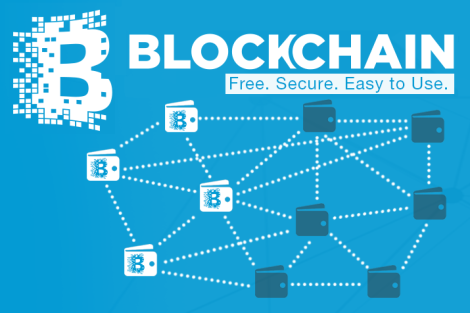
\includegraphics[width=0.95\textwidth]{img/d2si_blog_image_blockchain_wallet.png}
\end{minipage} \hfill \begin{minipage}[h]{0.75\textwidth}
	\textbf{Blockchain et les banques}~\\

	Qu'en est-il de la banque dans tout \c{c}a ? Eh bien, elle s'y int{\'e}resse de tr{\`e}s pr{\`e}s. Dans le contexte stressant de l'apr{\`e}s crise, de la mont{\'e}e des \texttt{comptes sans banque~\footnotemark} et des \texttt{Fintech~\footnotemark}, les banques  sont bien d{\'e}cid{\'e}es {\`a} ne pas manquer le cr{\'e}neau de la blockchain. Une \texttt{alliance sans pr{\'e}c{\'e}dent~\footnotemark} de neuf des plus grandes banques (dont Barclays, Goldman Sachs et JP Morgan) s'est cr{\'e}{\'e}e autour de cette technologie pour minimiser les co{\^u}ts de transaction. Mais l'innovation pourrait ne pas s'arr{\^e}ter l{\`a}. La blockchain pourrait {\'e}galement {\^e}tre utilis{\'e}e pour transmettre des contrats par exemple afin d'{\'e}viter tout litige ou afin de tracer l'activit{\'e} dans le cadre des audits. Aussi, ces innovations porteront avec elles d'autres secteurs d'activit{\'e} comme la s{\'e}curit{\'e}, le NoSql, voire le BigData au niveau de l'analyse et de l'exploitation des donn{\'e}es de la blockchain et du r{\'e}seau. Enfin, du c{\^o}t{\'e} des d{\'e}tracteurs, il convient de se poser la question de la consommation d'un tel syst{\`e}me qui immobilise une quantit{\'e} non n{\'e}gligeable de puissance de calcul, donc de consommation d'{\'e}nergie. Malgr{\'e} cela, pour Vitelik Buterin, fondateur d'\texttt{Ethereum~\footnotemark}, les blockchains pourraient g{\'e}rer \texttt{plusieurs milliards d'utilisateurs~\footnotemark} d'ici 5 ans.~\\
\end{minipage}
\footnotetext{\texttt{http://www.lemonde.fr/argent/article/2015/05/04/le-compte-sans-banque-fait-un-tabac\_4627124\_1657007.html}}
\footnotetext{\texttt{http://blog.d2-si.fr/2015/10/26/fintech/}}
\footnotetext{\texttt{http://www.itespresso.fr/blobkchain-banques-bitcoin-loin-107942.html}}
\footnotetext{\texttt{https://fr.wikipedia.org/wiki/Ethereum : Ethereum est une machine virtuelle fond{\'e}e sur les cha{\^i}nes de blocs (en anglais, blockchain) permettant la cr{\'e}ation par les utilisateurs de contrats intelligents gr{\^a}ce {\`a} un langage permettant de les programmer. Ces contrats intelligents sont bas{\'e}s sur un protocole informatique permettant de v{\'e}rifier ou de mettre en application un contrat mutuel, ils sont d{\'e}ploy{\'e}s sous la forme d'un blockchain. --- Ethereum utilise une monnaie, l'Ether, comme moyen de paiement de ces contrats. }}
\footnotetext{\texttt{http://www.lesechos.fr/tech-medias/medias/021617278405-vitalik-buterin-les-blockchains-gereront-des-milliards-dutilisateurs-dici-5-ans-1192256.php}}

\begin{minipage}[h]{0.23\textwidth}
	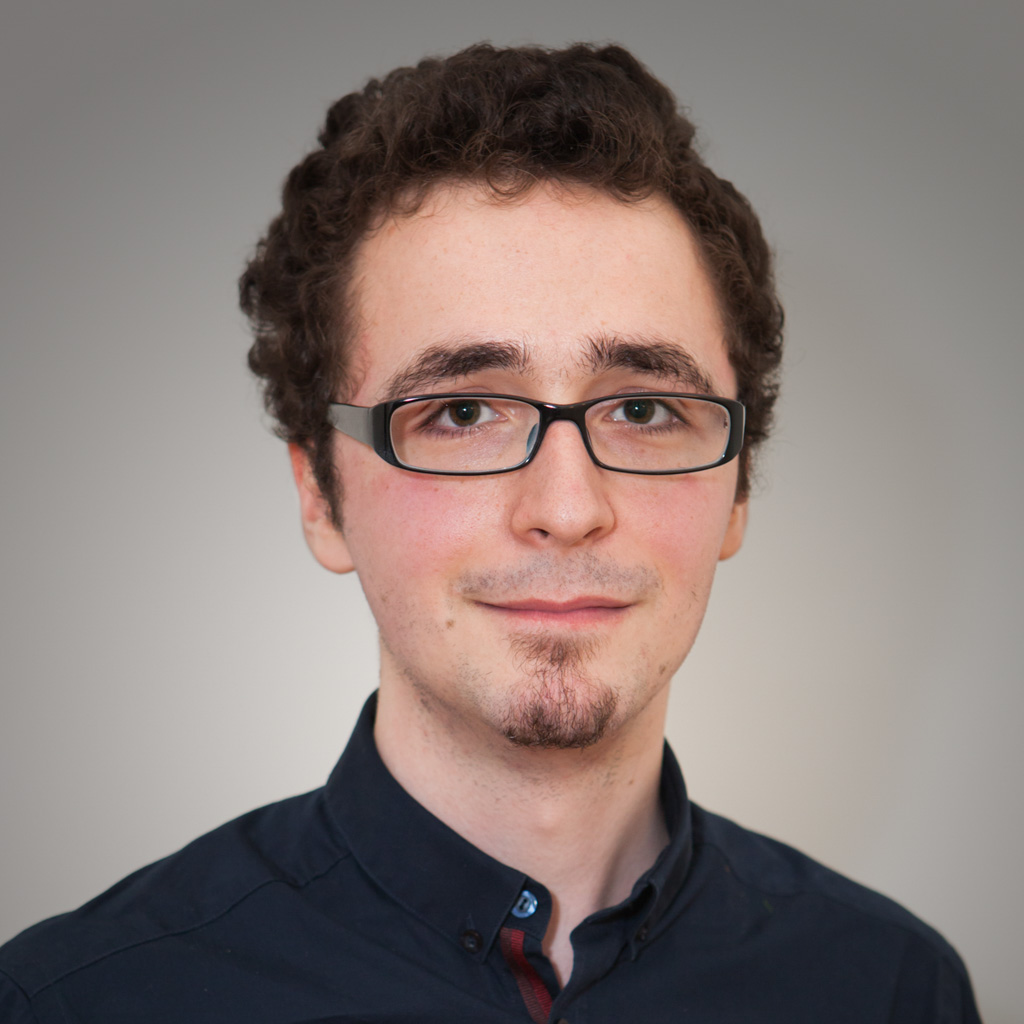
\includegraphics[width=0.95\textwidth]{img/d2si_blog_image_nicolas.jpg}
\end{minipage} \hfill \begin{minipage}[h]{0.75\textwidth}
	{\`A} propos de l'auteur~\\
	
	Apr{\`e}s son dipl{\^o}me de l'ENSIMAG, Nicolas Peray a rejoint D2SI afin de prendre en charge, entre autres, les logiciels internes de gestion indicielle dans une banque de financement. Discret mais curieux, il se revendique de la culture Geek en s'int{\'e}ressant {\`a} la technologie mais aussi {\`a} la culture, l'{\'e}ducation ou la psychologie.~\\
\end{minipage}

\clearpage

\texttt{\small http://www.lemonde.fr/argent/article/2015/05/04/le-compte-sans-banque-fait-un-tabac\_4627124\_1657007.html}~\\

\textbf{\Large Le compte sans banque fait un tabac}~\\
\emph{ LE MONDE ARGENT | 04.05.2015 {\`a} 14h55 --- Mis {\`a} jour le 07.05.2015 {\`a} 17h57 | Par Fr{\'e}d{\'e}ric Cazenave }~\\

\begin{minipage}[h]{0.23\textwidth}
	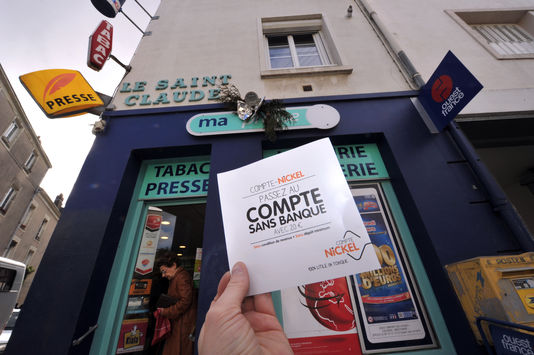
\includegraphics[width=0.95\textwidth]{img/4629281_6_a383_devant-un-bureau-de-tabac-nantais-en-fevrier_f32148e2c21cddc3f51a1bd877ad7d65.jpg} ~\\
	\emph{Devant un bureau de tabac nantais, en f{\'e}vrier 2014. le Compte-Nickel vient de franchir la barre des 100 000 clients.}~\\
\end{minipage} \hfill \begin{minipage}[h]{0.75\textwidth}
	Quatorze mois apr{\`e}s son lancement, le Compte-Nickel, ce compte bancaire un peu particulier qui s'ouvre en quelques minutes chez un des 1 000 buralistes partenaires, vient de franchir la barre des 100  000 clients. Au cours des trois premiers mois de l'ann{\'e}e, 27 000 personnes y ont adh{\'e}r{\'e}. Soit trois fois plus qu'au cours du premier trimestre de 2014. S'il remporte un tel succ{\`e}s, c'est qu'il permet {\`a} toutes les populations, m{\^e}me celles exclues du syst{\`e}me bancaire, de b{\'e}n{\'e}ficier d'une carte de paiement et de (relev{\'e}s d'identit{\'e} bancaire (RIB). Il suffit de 20 euros, d'une pi{\`e}ce d'identit{\'e} et d'un justificatif de domicile pour obtenir sa carte en cinq minutes chrono. ~\\

	<< \emph{Un quart de nos clients n'ont pas de revenus r{\'e}guliers ou sont sans emploi, explique Hugues Le Bret, un des fondateurs. Comme nous ne faisons pas de cr{\'e}dit et que nous ne permettons pas de d{\'e}couvert, nous ne demandons pas de fiche de paie et sommes moins intrusifs que les banques. Nous nous adressons {\`a} tout le monde, aux populations fragiles bien s{\^u}r, mais aussi {\`a} toux ceux qui veulent disposer d'un moyen de paiement {\`a} faible co{\^u}t. } >> ~\\
	<< \emph{Le co{\^u}t annuel du compte, estim{\'e} entre 30 et 50 euros, est au moins trois fois moins {\'e}lev{\'e} que dans une banque classique. } >> --- Ludovic Herschlikovitz, le fondateur du comparateur Choisir-ma-banque.com ~\\
\end{minipage}

Car c{\^o}t{\'e} tarif, et bien que chaque d{\'e}bit dans un distributeur automatique soit factur{\'e} 1 euro, << \emph{le co{\^u}t annuel du compte, estim{\'e} entre 30 et 50 euros, est au moins trois fois moins {\'e}lev{\'e} que dans une banque classique} >>, souligne Ludovic Herschlikovitz, le fondateur du comparateur Choisir-ma-banque.com. ~\\

Cette carte n'autorisant pas de d{\'e}couvert, elle {\'e}vite aussi de co{\^u}teuses p{\'e}nalit{\'e}s (commission d'intervention, agios...). << \emph{Gr{\^a}ce {\`a} notre technologie, nous sommes m{\^e}me capables lorsqu'un pr{\'e}l{\`e}vement va {\^e}tre effectu{\'e} de pr{\'e}venir le client si son compte n'est pas suffisamment cr{\'e}dit{\'e} afin qu'il puisse l'alimenter} >>, souligne M. Le Bret.  << \emph{Un compte bancaire ouvert {\`a} tous avec des tarifs tr{\`e}s comp{\'e}titifs  : ce que les banques n'ont jamais r{\'e}ussi, ou voulu faire, cette soci{\'e}t{\'e} y est parvenue. } >>, s'enthousiasme Maxime Chipoy, responsable des {\'e}tudes de l'association de consommateurs UFC-Que choisir. ~\\

\textbf{Second moyen de paiement} ~\\

Utilis{\'e}e comme compte principal par pr{\`e}s de trois quarts des clients, la carte sert aussi de second moyen de paiement pour les d{\'e}penses communes au sein d'un couple, dans le cadre de collocations, ou pour les achats sur Internet. <<  Comme il n'y a pas de d{\'e}couvert, les cons{\'e}quences d'un piratage sur le Web sont moindres, m{\^e}me si de toute fa\c{c}on le consommateur serait rembours{\'e} en cas de fraude sur sa carte  >>, pr{\'e}cise M Chipoy. Cette offre devrait aussi s{\'e}duire les {\'e}tudiants qui partent {\`a} l'{\'e}tranger, aucune commission de change, ni de frais suppl{\'e}mentaires n'{\'e}tant factur{\'e}s. --- Et pour les parents tent{\'e}s d'{\'e}quiper leurs enfants, sachez qu'une offre destin{\'e}e aux plus de 12 ans sera lanc{\'e}e {\`a} l'automne. ~\\

Les buralistes, eux aussi, y trouvent leur int{\'e}r{\^e}t. Ils touchent 3 euros pour chaque dossier ouvert et sont r{\'e}mun{\'e}r{\'e}s lors des d{\'e}p{\^o}ts ou des retraits d'esp{\`e}ces. << \emph{Un professionnel qui ouvre en moyenne un compte par jour gagne au bout de trois ans 640 euros par mois. Cela repr{\'e}sente 10 \% de son revenu annuel. A Paris, nous avons un bureau de tabac qui parvient {\`a} faire ouvrir tellement de comptes que cette nouvelle activit{\'e} lui rapporte 2  000 euros par mois. } >>, avance M. Le Bret. --- De quoi inciter le nombre d'officines {\`a} s'{\'e}quiper -- 1 400 le seront en fin d'ann{\'e}e, soit moins de 5 \% du nombre total -- et permettre au Compte-Nickel de poursuivre sur sa lanc{\'e}e. M. Le Bret esp{\`e}re atteindre 220  000 clients fin 2015. ~\\

Pour trouver les buralistes partenaires : Compte-nickel.fr ~\\

\end{document}
